\documentclass[11pt]{article}
\usepackage[margin=1in]{geometry}
\usepackage{amsmath,amssymb}
\usepackage{lmodern}
\usepackage[T1]{fontenc}
\usepackage{enumitem}
\usepackage{microtype}
\usepackage{tikz}
\usetikzlibrary{arrows.meta,angles,quotes,calc,decorations.pathreplacing}

\title{2017 F=ma Exam Review}
\author{Nathan P.}
\date{December 28, 2025}

\begin{document}
\maketitle

\section*{Problem 2}
The box $M$ also oscillates when it's in free fall.
If 2 masses oscillate on one spring, $\omega^2=k/\mu$ where $\mu=\dfrac{Mm}{M+m}$:
\[
\omega=\sqrt{\frac{k(M+m)}{Mm}}=\sqrt{k\left(\frac1m+\frac1M\right)},
\]
which is greater than the initial $\omega=\sqrt{k/m}$.
Key idea: the relative acceleration of the mass in the box's frame is
\[
a_{\text{mass}}-a_{\text{box}}=-\frac Fm-\frac FM=-kx\left(\frac1m+\frac1M\right),
\]
which is in the form $\ddot x=-\omega^2x$, so $\omega=\sqrt{k(1/m+1/M)}$, which is greater than the initial.
In general, free-free systems oscillate faster than fixed-free systems.

\section*{Problem 3}
There are no external horizontal forces, so the horizontal com position stays the same.

\section*{Problem 6}
Treat the connected bars as one object, so the internal tensions cancel. Then be careful with the acting distances and solve for $M_3$.

\section*{Problem 7}
It asks for
\[
\frac{dK}{dt}=\frac{\tfrac12mv^2}{t}=\tfrac12\rho v^2,\qquad \rho=\frac{dm}{dt}.
\]
This is not the same as $P=\Delta E/t$ because there is variable mass.

\section*{Problem 8}
$P=Fv$ and $F=\dfrac{dm}{dt}v=\rho v$, so $P=\rho v^2$. ($dm/dt$ is generally written as $\dot m$, so $P=\dot mv^2$.)

\section*{Problem 9}
Tricky, because you might think $P=\rho gh$, $F=PA=\rho ghA=\rho gV=$ constant, since it said the same volume is poured into each flask. NO. $hA\neq V$ because $h$ is not constant for each.
Instead, $P=\rho gh$ and $h_C>h_A>h_B$ intuitively. $F=PA$, so $F\propto P\propto h$, so it's that same order.

\section*{Problem 10}
Key idea: you can use various vertical paths to compute the pressure at a certain depth.
There's no $P_{\text{atm}}$ at the top of the handle.
\[
P_{\text{bottom}}=P_{\text{atm}}+\rho gH=\rho gh+P_{\text{top of handle}},\qquad
P_{\text{gauge}}=P_{\text{bottom}}-P_{\text{atm}}=\rho gH.
\]
A follow-up question might be: what's the pressure at the top of the handle? It would just be $P_{\text{atm}}+\rho g(H-h)$.

\section*{Problem 13}
$a=\dfrac{M-m}{M+m}g$. With one side super heavy, $a$ approaches $g$.
For the light side to accelerate up at $g$, there must be an upward force of $2mg$ for the net force to be $mg$ upward.

\section*{Problem 14}
Rolling without slipping means $f$ varies, so the acceleration of the com is NOT the same for all of them.
\begin{enumerate}[leftmargin=*, itemsep=0.25em]
\item $a_{cm}=\dfrac{g\sin\theta}{1+c}$, where $c$ is the fraction before $MR^2$ in the $I$ value, so less $I$ means greater $a$.
\item Alternatively, think energy. $E_i=E_f$, $U_i=K_t+K_r$. $K_r\propto I$, so less $I$ means less energy ``wasted'' rotating, and $K_t$ will end greater, implying greater acceleration.
\end{enumerate}

\section*{Problem 16}
Key idea: the length of the rod is unchanging. Conservation of length, $\Delta L=0$, means $\Delta v=0$ along the rod.
Using this fact, find the components along the rod: $v\cos\theta$ and, with some geometry, $u\cos(\alpha-\theta)$. Set them equal ($v$ must be the same parallel to the rod).

\section*{Problem 19}
Note that it is a speed vs.\ time graph and the graph is not numerically labeled, so we're probably dealing with ratios (we don't have actual values for acceleration, just their ratio).
Since speed is the magnitude of velocity, the slope is NOT acceleration with direction. We're taking ratios of the magnitude of acceleration, so we should take the ratio of the magnitude of the force up and down the incline to get a correct result.
Since acceleration is related to force, we can sum the forces twice, going up and going down the incline, and divide out mass to get the two acceleration expressions. Divide those to get the same ratio as the slopes, set it equal to the ratio of the slopes, and we're left with an expression with $g$, $\mu$, and $\theta$. We're given $\theta$, so solve for $\mu$.
The graph is not labeled with units, so we can't have a definite acceleration value.

\section*{Problem 22}
You can solve this either the math way or the physics way.
Physics way: energy is conserved. You cannot transfer more than 100\% of the energy, so the fractional energy transfer can be no greater than 1. The only way to transfer all the kinetic energy is the classic elastic collision where the first particle transfers all its momentum to a second particle of equal mass.
Math way: $K_f/K_i$ becomes
\[
\frac{4Mm}{M^2+2Mm+m^2},
\]
and the answer options show $m/M$, so set $r=m/M$ and divide the top and bottom by $Mm$. The bottom has $r+1/r$ added, so you have to minimize that. Take the derivative, set it to $0$, and solve: $r=1$, so $m=M$.
Learned: in general, if $m$ has an elastic collision with a stationary $M$, the max momentum $M$ gets is twice the momentum of the initial moving mass, and the max kinetic energy $M$ gets is 100\% of $m$'s initial KE.

\section*{Problem 24}
The setup is standard; the easy thing to forget is that the $K$ of both objects is $\tfrac12(M+m)v'^2$, not just $\tfrac12mv'^2$. Combining $K_i-K_f$ you'll eventually get
\[
1-\frac{m}{m+M}=\frac{M+m-m}{m+M}=\frac{M}{M+m},
\]
and the math works out to the answer.
You can also rule out C, D, and E, because when $M\to\infty$ it's basically $\tfrac12mv^2=\tfrac12kx^2$, $x=v\sqrt{m/k}$, and C, D, E don't approach that limit. B can be ruled out because it doesn't depend on $M$.

\section*{Problem 25}
Use geometry and vis-viva to get an expression for $v_2/v_1$.
The distance $SP$ plus the distance from $P$ to the other focus should equal $2a$ (for a satellite on an ellipse, the distances to the two foci add to $2a$).
Vis-viva, $v^2=GM\left(\dfrac2r-\dfrac1a\right)$, with $SP$ as $r_1$:
\[
\frac{v_2^2}{v_1^2}=\frac{2/r_2-1/a}{2/r_1-1/a}.
\]

\begin{center}
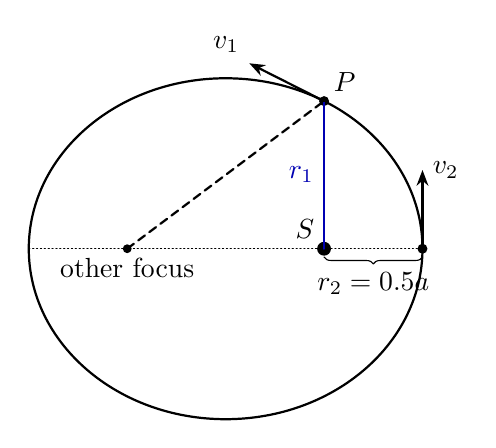
\begin{tikzpicture}[scale=1.0, line cap=round, line join=round, >={Stealth[length=2mm]}]
  % a = 2.5, perigee 0.5a -> c = 1.25, b = 2.165; P = (c, b^2/a) = (1.25, 1.875)
  \draw[thick] (0,0) ellipse (2.5 and 2.165);
  \draw[densely dotted] (-2.5,0) -- (2.5,0);
  \fill (1.25,0) circle (2.5pt) node[above left] {$S$};
  \fill (-1.25,0) circle (1.6pt) node[below] {other focus};
  \fill (1.25,1.875) circle (1.8pt) node[above right] {$P$};
  \fill (2.5,0) circle (1.8pt);
  \draw[thick, blue!70!black] (1.25,0) -- (1.25,1.875) node[midway, left] {$r_1$};
  \draw[thick, densely dashed] (-1.25,0) -- (1.25,1.875);
  \draw[decorate, decoration={brace, mirror, raise=3pt}] (1.25,0) -- (2.5,0) node[midway, below=5pt] {$r_2=0.5a$};
  \draw[->, thick] (2.5,0) -- (2.5,1.0) node[right] {$v_2$};
  \draw[->, thick] (1.25,1.875) -- ++(-0.95,0.48) node[above left] {$v_1$};
\end{tikzpicture}
\end{center}

\end{document}
